
%%%%%%%%%%%%%%%%%%%%%%%%%%%%%%%%%%%%%%%%%
% University Assignment Title Page 
% LaTeX Template
% Version 1.0 (27/12/12)
%
% This template has been downloaded from:
% http://www.LaTeXTemplates.com
%
% Original author:
% WikiBooks (http://en.wikibooks.org/wiki/LaTeX/Title_Creation)
%
% License:
% CC BY-NC-SA 3.0 (http://creativecommons.org/licenses/by-nc-sa/3.0/)
% 
% Instructions for using this template:
% This title page is capable of being compiled as is. This is not useful for 
% including it in another document. To do this, you have two options: 
%
% 1) Copy/paste everything between \begin{document} and \end{document} 
% starting at \begin{titlepage} and paste this into another LaTeX file where you 
% want your title page.
% OR
% 2) Remove everything outside the \begin{titlepage} and \end{titlepage} and 
% move this file to the same directory as the LaTeX file you wish to add it to. 
% Then add \input{./title_page_1.tex} to your LaTeX file where you want your
% title page.
%
%%%%%%%%%%%%%%%%%%%%%%%%%%%%%%%%%%%%%%%%%
%\title{Title page with logo}
%----------------------------------------------------------------------------------------
%	PACKAGES AND OTHER DOCUMENT CONFIGURATIONS
%----------------------------------------------------------------------------------------

\documentclass[23pt]{article}
\usepackage[margin=1in, paperwidth=21cm, paperheight=29.7cm]{geometry}
\usepackage[pdftex]{color,graphicx}
\usepackage[english]{babel}
\usepackage[utf8x]{inputenc}
\usepackage{amsmath}
\usepackage[colorinlistoftodos]{todonotes}
\usepackage{cite}
\usepackage{listings}
\usepackage[nodayofweek]{datetime}
\usepackage{setspace}
\usepackage{fancyhdr}
\usepackage{tabu}
\newcommand{\HRule}{\rule{\linewidth}{0.5mm}}
\newcommand{\abbrlabel}[1]{\makebox[5cm][l]{\textbf{#1}\ \dotfill}}
\newenvironment{abbreviations}{\begin{list}{}{\renewcommand{\makelabel}{\abbrlabel}}}{\end{list}}
\begin{document}
\nocite{*}
\pagenumbering{roman}
\title{\begin{center}
\bf SEMINAR REPORT\\
\vspace{0.5cm} On\\
\HRule \\[0.4cm]
{ \huge \bfseries Bio Computers}\\[0.4cm] % Title of your document
\HRule \\[0.4 cm]
\vspace{0.5cm} \begin{Large} Submitted by:\\ 
\vspace{.35cm}Vinod Kumar S (13400061)
\end{Large}
\end{center}}
\vspace{.5cm}
\date{}

\maketitle
\begin{center}
 {\it\large for the award of the degree}
\end{center}
\begin{center}
 {\it\large of}
\end{center}
\begin{center}
 {\bf\Large Bachelor of Technology}
\end{center}

\begin{center}

\includegraphics[scale=.8]{images/logo.jpg}
\end{center}
\vspace{.28cm}

\begin{center}
{\bf\large DEPARTMENT OF COMPUTER SCIENCE AND ENGINEERING}

\vspace{.35cm}
{\bf\large COLLEGE OF ENGINEERING\ , TRIVANDRUM}
\begin{center}{\large \formatdate{19}{7}{2016}}\\[1cm]\end{center}
\end{center}

\newpage

\begin{center}
{\bf{\LARGE CERTIFICATE}}
\end{center}
\vspace{.1cm}
\begin{center}

\includegraphics[scale=.45]{images/logo.jpg}
\end{center}
\begin{center}
\textbf{\Large College of Engineering,
Trivandrum}
\end{center}

\vspace{.6cm}
\begin{Large}
\begin{spacing}{1.5}
\hspace{1.5cm} This  is  to certify that the seminar entitled {\bf Bio Computers} done by {\bf  Vinod Kumar S (13400061)} of the {\bf Department of Computer Science and Engineering, College of Engineering, Trivandrum} in partial fulfillment of the requirements for the award of the degree of Bachelor of Technology in Computer Science and Engineering under Kerala University is a Bonafide record of work carried out by him.
\vspace{2cm}
\end{spacing}

\bf\Large \hspace{.3cm}\hspace{1.7cm} \hspace{3cm} \\
\bf\Large \hspace{1cm}Seminar Co-ordinator    \hspace{4cm} Head of Department

\vspace{2cm}
\begin{spacing}{1.4}
\noindent Place : Trivandrum

\noindent Date \ : \formatdate{25}{7}{2016}
\end{spacing}
\end{Large}

\newpage
\pagenumbering{roman}
\begin{center}
\bf{{\LARGE ACKNOWLEDGEMENT}}
\end{center}
\begin{Large}
\begin{spacing}{1.1}
\vspace{1cm}
\hspace{2cm}
It is with great enthusiasm and spirit I am bringing out this seminar report. First of all I thank the God Almighty for His grace and mercy that enabled me in the finalization of this seminar.

\hspace{2cm} 
I am greatly obliged to Dr. Abdul Nizar, Head Of the Department of Computer Science,  College of Engineering, Trivandrum, for his encouragement and support. I am immensely indebted to our seminar coordinators Mr. Vipin Vasu A. V. and Mr. Sreelal S. , for their constructive criticisms, guidance and advices. I, on this occasion, remember the valuable suggestions and prayers offered by my family members and friends which were inevitable for the successful completion of my seminar.
\end{spacing}
\end{Large}
\newpage
\begin{center}{\bf{\LARGE ABSTRACT}}
\end{center}
\begin{Large}
\begin{spacing}{1.1}
Biocomputing is one of the upcoming field in the areas of molecularelectronics and nanotechnology. The idea behind blending biology with technology is due to the limitations faced by the semiconductor designers in decreasing the size of the silicon chips, which directly affects the processor speed. Biocomputers consists of biochips unlike the normal computers, which are silicon-based computers. This biochip consists of biomaterial such as nucleic acid, enzymes, etc.

The power of a biocomputer is that it acts as a massively parallel computer and has immense data storage capability. Thus, it can be used to solve NP-complete problems with higher efficiency. The possibilities for biocomputers include developing a credit card size computer that could design a super-efficient global air-traffic control system. The basic idea behind biocomputing is to use molecular reactions for computational purposes.
\end{spacing}
\end{Large}

\newpage
\tableofcontents
\listoffigures
\newpage

\textbf{Abbrevations}
\begin{abbreviations}
\item[DNA] Deoxyribo Nucleic acid
\item[RNA] Ribo Nucleic acid
\item[HPP] Hamiltonion Path Problem
\item[NP] Nondeterministic Polynomial time
\item[PCR] Polymerase  Chain  Reaction
\item[DES] Data Encryption Standard 

\end{abbreviations}
\newpage
\renewcommand{\abstractname}{\Large Abstract}
	
\newpage
\pagenumbering{arabic}
\section{Introduction}
\label{sec:introduction}

Biocomputers use systems of biologically derived molecules- such as DNA and proteins to perform computational calculations involving storing, retrieving and processing data.

DNA  (Deoxyribo Nucleic  Acid)  computing,  also  known  as  molecular 
computing is a new approach to massively parallel computation based on 
groundbreaking  work  by  Adleman.  DNA  computing  was  proposed  as  a 
means of solving a class of intractable computational problems in which
the  computing  time  can  grow  exponentially  with  problem  size  (the  `NP
- complete' or non-deterministic polynomial time complete problems) .
A  DNA  computer  is  basically  a  collection  of  specially  selected  DNA 
strands whose combinations will result in the solution to some problem, depending  on  the  problem  at  hand.  Technology  is  currently  available both  to  select  the  initial  strands  and  to  filter  the  final  solution.

DNA computing is a new computational paradigm that employs (bio) molecular 
manipulation   to   solve   computational   problems,   at   the   same   time exploring  natural  processes  as  computational  models.  In  1994, 
Leonard Adleman at the Laboratory of Molecular   Science, Department of Computer Science, University   of   Southern   California   surprised   the 
scientific  community  by  using  the  tools  of  molecular  biology  to  solve  a different computational problem. 

\section{DNA Computing}
\label{sec:theory}

\subsection{DNA Fundamentals}
DNA (deoxyribonucleic acid) is a double stranded sequence of 4 nucleotides. The four nucleotides that compose a strand of deoxyribonucleic acid are as
follows: Adenine (A), guanine (G), Cytosine (C) and Thymine (T): they are typically referred to as bases. The order of those bases is what determines DNA’s instructions, or ordering.

DNA performs two major functions:
  \begin{itemize}
    \item self replication.
        \item codes for production of proteins.
  \end{itemize}
Each deoxyribonucleotide consists of 3 components:
  \begin{itemize}

  \item {a sugar — deoxyribose.
      \begin{itemize}
      \item five carbon atoms: 1' to 5'.
      \item hydroxyl group (OH) attached to 3' carbon.
    \end{itemize}}
  \item a phosphate group.
  \item a nitrogenous base.
\end{itemize}

% \begin{figure}
%     \includegraphics[width=\textwidth]{dnaBases}
%   \caption{\label{fig:dnaBases}DNA structure}
% \end{figure}

\begin{figure}[h!]
  \centering
  \includegraphics[width=0.8\textwidth]{images/dnaBases}
  \caption{DNA Bases}
\end{figure}

The chemical structure of deoxyribonucleic acid consists of a specific bond of 2 linear sequences of bases. This bond follows a property of Complementarity: adenine bonds with T (A-T) and vice-verse (T-A), cytosine bonds with G (C-G) and vice-verse (G-C). This is called Watson-Crick complementarity.
% new line
The four nucleotides adenine (A), guanine (G), cytosine (C) and thymine (T) compose a strand of DNA. The polarity of DNA strands is determined by its two different ends: the 3’end, and the 5’end. The double helix is an anti-parallel (two strands of opposite polarity) bonding of two complementary strands.

\begin{figure}[h!]
  \centering
  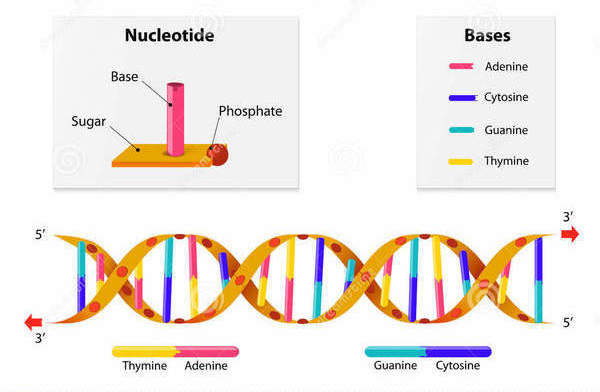
\includegraphics[width=\textwidth]{images/dna}
  \caption{DNA Structure}
\end{figure}
 
\subsection{Basic Operations on DNA}
DNA is the major data storage molecule in living cells. There are highly  specific  enzymes  that  can  either duplicate the information in DNA molecules or transmit this information to other DNA molecules. Instead of using electrical impulses to represent bits of  information, the  DNA  computer  uses  the  chemical  properties  of these  molecules by  examining  the  patterns  of  combination  or  growth  of the  molecules or  strings.  DNA  can  do  this  through  the  manufacture  of enzymes, which   are   biological   catalysts that are analogous to `software' for computing data.

A single strand of DNA is string that consists of four different symbols A, C, G, T. Mathematically this means we have at our disposal a  letter alphabet, $\sum$=\{A T G C\} to encode information. In a DNA computer, computation takes place in test tubes or on a glass slide coated in 24K gold. The input and output  are  both strands  of  DNA,  whose  genetic  sequences  encode certain  information. A  program  on  a  DNA  computer  is  executed  as  a series  of  biochemical operations,  which  have  the  effect  of  synthesizing, extracting, modifying and cloning the DNA strands.
\\ \\

DNA computation are based on various combinations of the following primitive bio-operations:
  \begin{itemize}
    \item \textbf{Synthesizing}- A desired polynomial length strand is generated.
        \item \textbf{Mixing}- Combining the content of two test tubes to perform union operation.
        \item \textbf{Annealing}- bond  together  two  single-stranded  complementary  DNA sequences  by  cooling  the  solution.
        \item \textbf{Melting}- break apart a double-stranded DNA into its single-stranded complementary  components  by  heating  the  solution.
         \item \textbf{Amplifying (copying) }- make  copies  of  DNA  strands  by  using  the Polymerase  Chain  Reaction  (PCR).  The  DNA  polymerase  enzymes perform several   functions   including replication of DNA. The replication reaction requires a  guiding  DNA  single strand  called template and  a  shorter  oligonucleotide  called  a primer, that  is annealed to it. 
         \item \textbf{Separating}- Strands are separated by length using gel electrophoresis.
         \item \textbf{Extracting}- those strands that contain a given pattern as a substring by using affinity purification.
        \item \textbf{Ligating}- paste  DNA  strands  with  compatible  sticky  ends  by  using DNA  ligases.  Indeed,  another  enzyme  called DNA  ligase,  will  bond together, or ``ligate'', the end of a DNA strand to another strand.
        \item \textbf{Cutting}- DNA double-strands at specific sites by using commercially available   restriction   enzymes. One   class   of   enzyme, called restriction endonucleases, will recognize a specific short sequence of DNA,  known  as  a  restriction  site.  Any  double-stranded  DNA  that contains the restriction site within its sequence is cut by the enzyme at that location. 
        \item \textbf{Substituting}- substitute,  insert  or  delete  DNA  sequences  by  using PCR site-specific oligonucleotide mutagenesis.
        \item \textbf{Marking}- single strands by hybridization: complementary sequences are  attached  to  the  strands,  making  them  double-stranded.  The reverse    operation    is \textbf{unmarking} of    the    double-strands    by denaturing,  that  is,  by  detaching  the  complementary  strands.  The marked sequences will be double-stranded while the unmarked ones will be single-stranded.
        \item \textbf{Detecting and Reading}- given the contents of a tube, say ``yes'' if it contains at least one DNA strand, and ``no'' otherwise. PCR may be used  to  amplify  the  result  and  then  a  process  called \textbf{sequencing} used to actually read the solution. 
  \end{itemize}
    
    In short, the DNA computer encodes the problem to be solved in the DNA using the four values A, T, C, G. The solution to a problem is obtained as a DNA strand.
    
    Every  possible  sequence  can  be  chemically  created  in  a  test  tube  on trillions  of different  DNA strands and  the  correct  sequences  can  be filtered out using genetic engineering tools.
    
\subsection{DNA Computing Example - The Hamiltonion Path Problem}

In  1994  Leonard  M.  Adleman showed  how  to  solve  the  Hamilton  Path Problem, using DNA computation.
\\ \\
\textbf{Hamiltonion Path Problem:}

A directed graph G with designated nodes \textit{start} and \textit{end} is said to have a Hamiltonian  path  if  and  only  if  there  exists  a  sequence  of  compatible one-way  edges e1,e2,  ...en that  begins  at \textit{start},  ends  at \textit{end} and  enters every  other  node  exactly  once.  A  simplified  version  of  this  problem, known  as  the  traveling  salesman  problem,  poses  the  following  question: given  an  arbitrary  collection  of  cities  through  which  a  salesman  must travel, what is the shortest route linking those cities?

This problem is difficult for conventional computers to solve because it is a  ”non-deterministic  polynomial  time  problem”.  These  problems,  when the  instance  size  is  large,  are  intractable  with  conventional  computers, but   can   be   solved   using   massively   parallel   computers   like   DNA computers.     NP     problems     are     intractable     with     deterministic (conventional/serial)   computers,   but   can   be   solved   using   non-deterministic (massively parallel) computers. A DNA computer is a type of non-deterministic  computer.  The  Hamiltonian  Path  problem  was  chosen by Adleman because it is known as ”NP-complete”.
  \begin{figure}[h!]
    \centering
      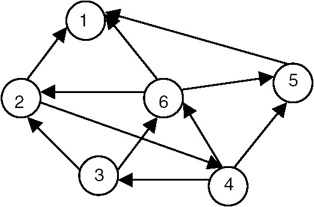
\includegraphics[width=\textwidth]{images/graphHPP}
      \caption{Directed graph with node 4 as source(start) and node 1 as destination node(end)}
  \end{figure}
    \\ \\ \\
  \begin{figure}
      \centering
      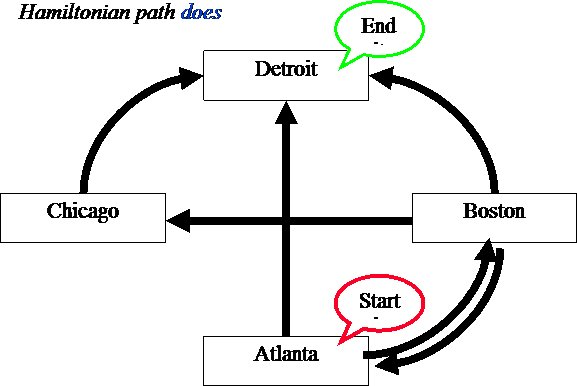
\includegraphics[width=\textwidth]{images/hpp_converted}
      \caption{Simplified Graph - Hamiltonion Path is Atlanta-Boston-Chicago-Detroit}
  \end{figure}
\textbf{Adleman's Algorithm}
\\ \\ 
\textbf{Input:} A directed graph G with n vertices, and designated vertices start and end.
\\
\textbf{Step 1:} Generate paths in G randomly in large quantities.
\\
\textbf{Step 2:} Reject all paths that 
\begin{itemize}
  \item do not begin with start.  
  \item do not end in end.
\end{itemize}
\textbf{Step 3:} Reject all paths that do not involve exactly n vertices.
\\
\begin{figure}[h!]
    \centering
      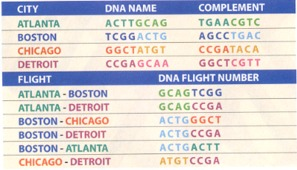
\includegraphics[width=0.7\textwidth]{images/table}
      \caption{DNA for vertices and edges}
  \end{figure}
\hspace{-4.1pt}\textbf{Step 4:} For each of the n vertices v:
\begin{itemize}
  \item reject all paths that do not involve v.
\end{itemize}
\textbf{Output:} YES, if any path remains; NO, otherwise.
\\ \\ 
\textbf{For step 1}, each node of the graph is encoded into a random 20-base strand of DNA. Then, for each edge of the graph, a different 20-base  oligonucleotide  was  generated  that  contains  the  second  half  of  the source code plus the first half of the target node.
\\
\textbf{To implement step 2}, the product of step 1 was amplified by PCR using oligonucleotide  primers  representing start and end  and  ligase  enzyme. This  amplified  and  thus  retained  only  those  molecules  encoding  paths that  begin  with start and  end  with end. 10\textsuperscript{14} computations  are  carried out in a single second.
\\
\textbf{For   implementing   step   3}, gel   electrophoresis   is used for the  separation and recovery of DNA strands of the correct length. The desired path, if it exists, would pass through all four nodes, each of which was assigned a length of 20 bases.
\\
\textbf{Step  4} is  accomplished  by  successive  use  of  affinity  purification  for each node other than the start and end nodes.

The solution strand has to be filtered from the test tube:

\textbf{GCAG TCGG ACTG GGCT ATGT CCGA}

Atlanta $\rightarrow$ Boston $\rightarrow$ Chicago $\rightarrow$ Detroit
\\ \\
For a  graph  with  n  vertices,  there  are  a  possible  (n-1)! permutations of the vertices between beginning and ending vertex. To  explore  each  permutation,  a  conventional  computer  must  perform O(n!)  operations  to  explore  all  possible  cycles.  However,  the  DNA computing model only requires the representative oligos. Once placed in  solution,  those  molecules  will  anneal  in  parallel,  providing  all  possible paths  in  the  graph  at  roughly  the  same  time.  That  is  equivalent  to O(1)  operations,  or  constant  time.  In  addition,  no  more  space  than what  was  originally  provided  is  needed  to  contain  the  constructed paths.

\section{Bio Computers}
\subsection{DNA Data Storage}
A DNA storage system consists of a DNA synthesizer that encodes the data to be stored in DNA, a storage container
with compartments that store pools of DNA that map to a volume, and a DNA sequencer that reads DNA sequences
and converts them back into digital data. Figure \ref{fig:system-overview} shows an overview of the integrated system.

The basic unit of DNA storage is a DNA strand that is roughly 100-200 nucleotides long, capable of storing 50-100
bits total. Therefore, a typical data object maps to a very large number of DNA strands. The DNA strands will be stored in
``pools'' that have stochastic spatial organization and do not permit structured addressing, unlike electronic storage media. Therefore, it is necessary to embed the address itself into the data stored in a strand. This way, after sequencing, one can reassemble the original data value.
\\ \\
\begin{figure}[h!]
    \centering
      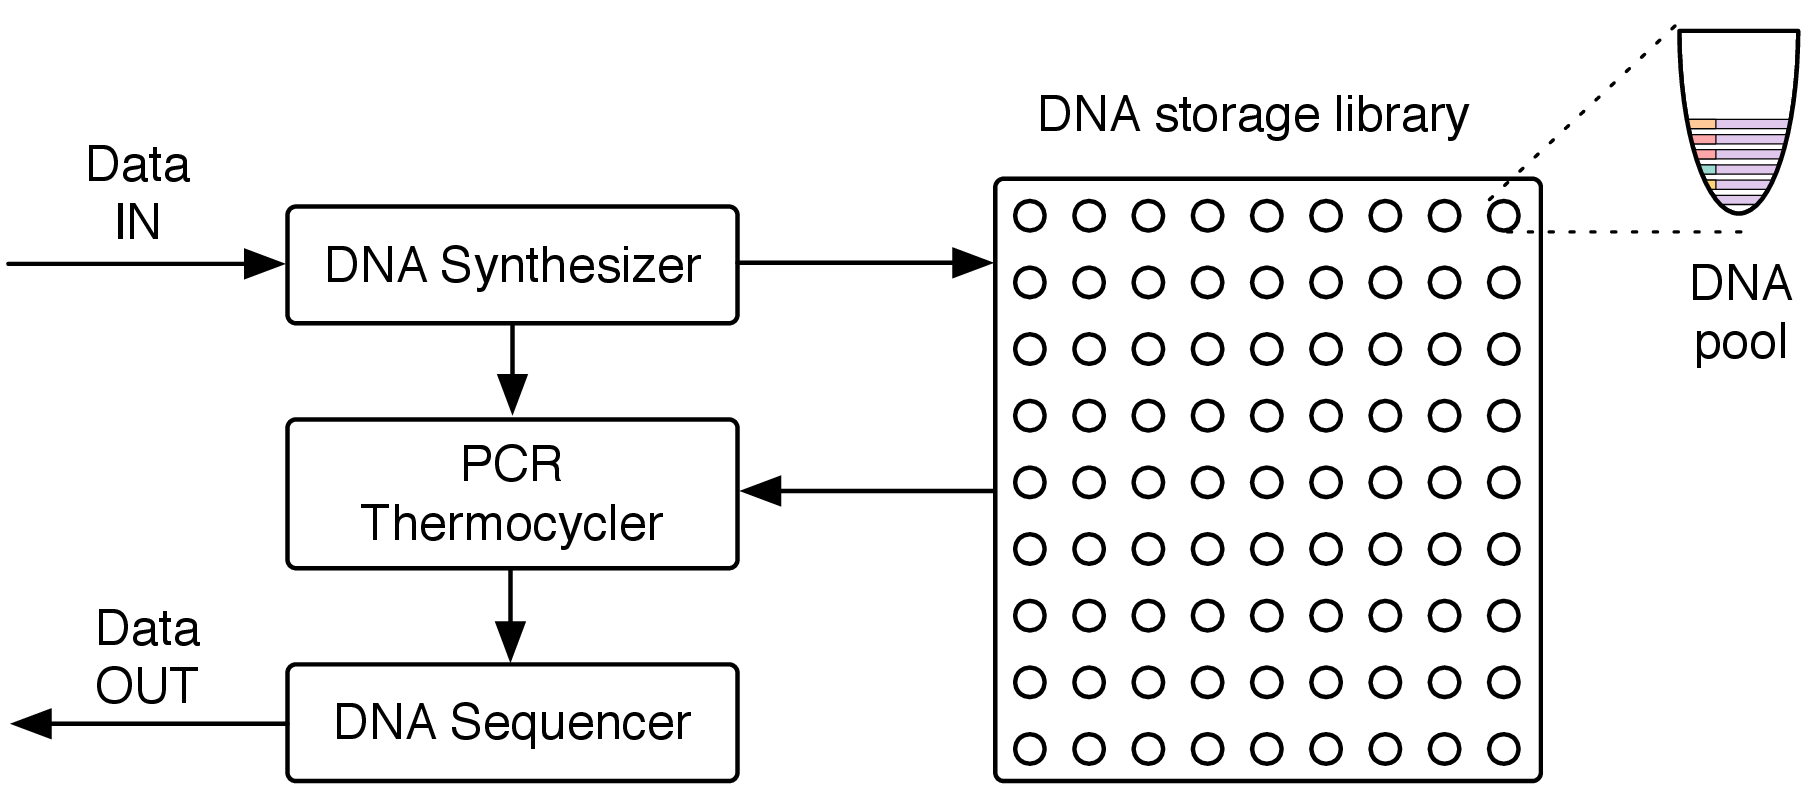
\includegraphics[width=0.7\textwidth]{images/system-overview}
      \caption{DNA Storage System Overview}
      \label{fig:system-overview}
  \end{figure}
\\
A storage system needs a way to assign identification tags to data objects so they can be retrieved later. A simple key-value architecture is used, where a \textit{put(key, value)} operation associates value with key, and a \textit{get(key)} operation retrieves the value assigned to key. To implement a key-value interface in a DNA storage system, there is : (1) a function that maps a key to the DNA pool (in the library) where the strands that contain data reside; and (2) a mechanism to selectively retrieve only desired portions of a pool (i.e, random access), since the DNA container will likely store significantly more data than the desired object.

Random access is implemented by mapping a key to a pair of PCR primers. At write time, those primers are added to the strands. At read time, those same primers are used in PCR to amplify only the strands with the desired keys. 

\begin{figure}[h!]
    \centering
      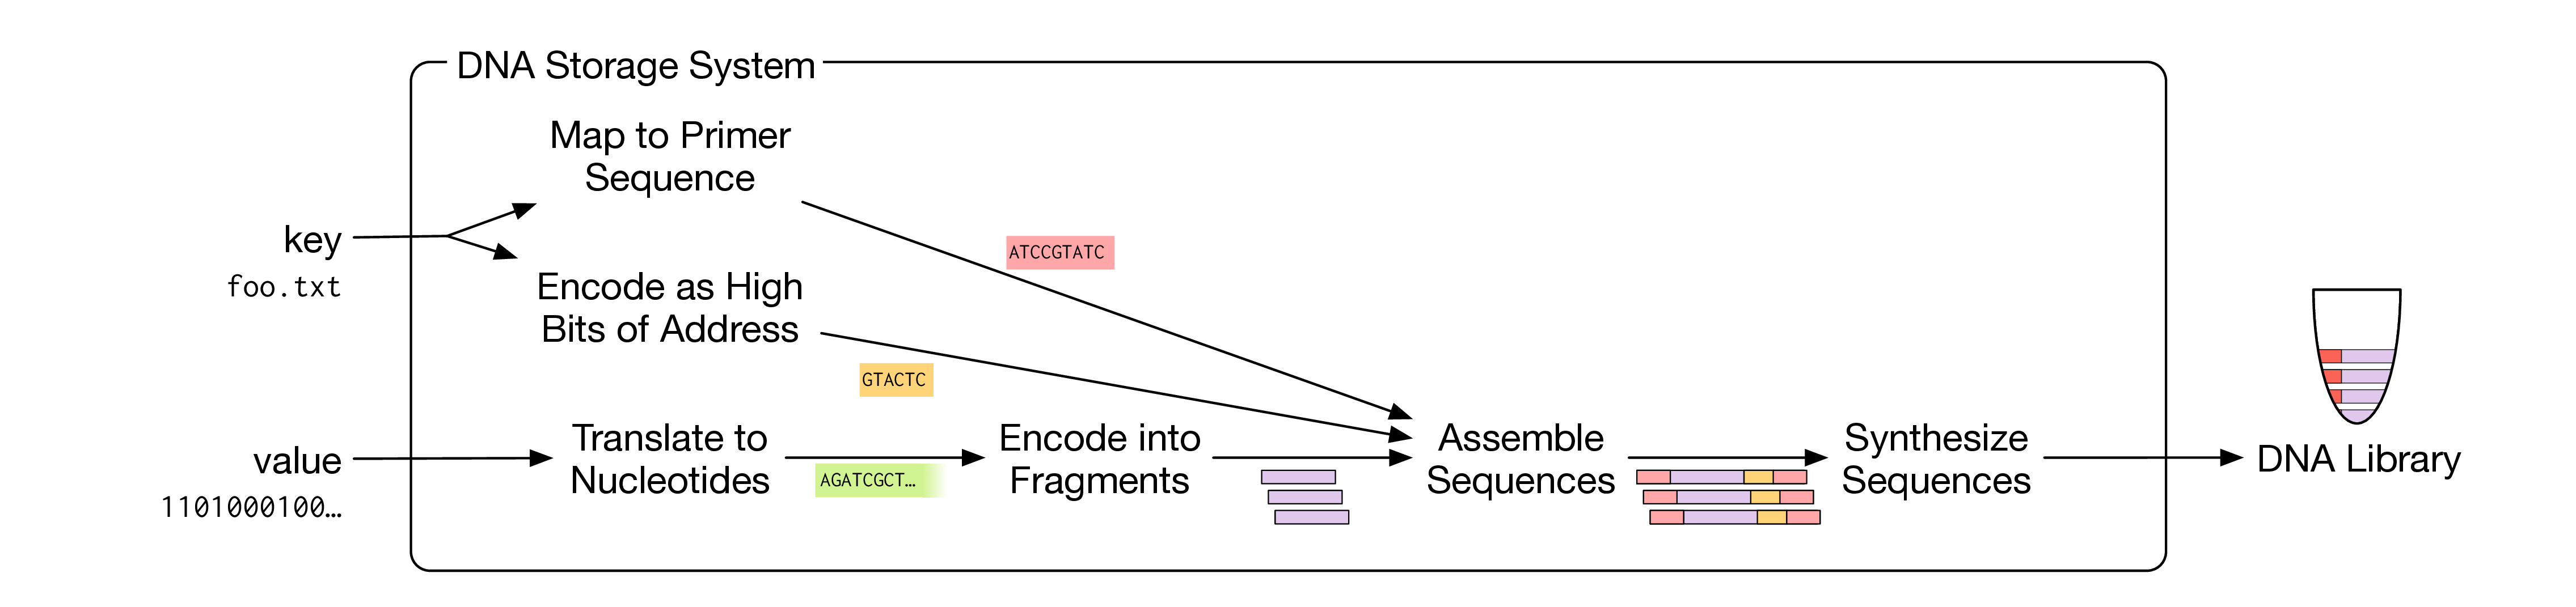
\includegraphics[width=1.1\textwidth]{images/write}
      \caption{DNA Storage System Write}
      \label{fig:write}
  \end{figure}
  \begin{figure}[h!]
    \centering
      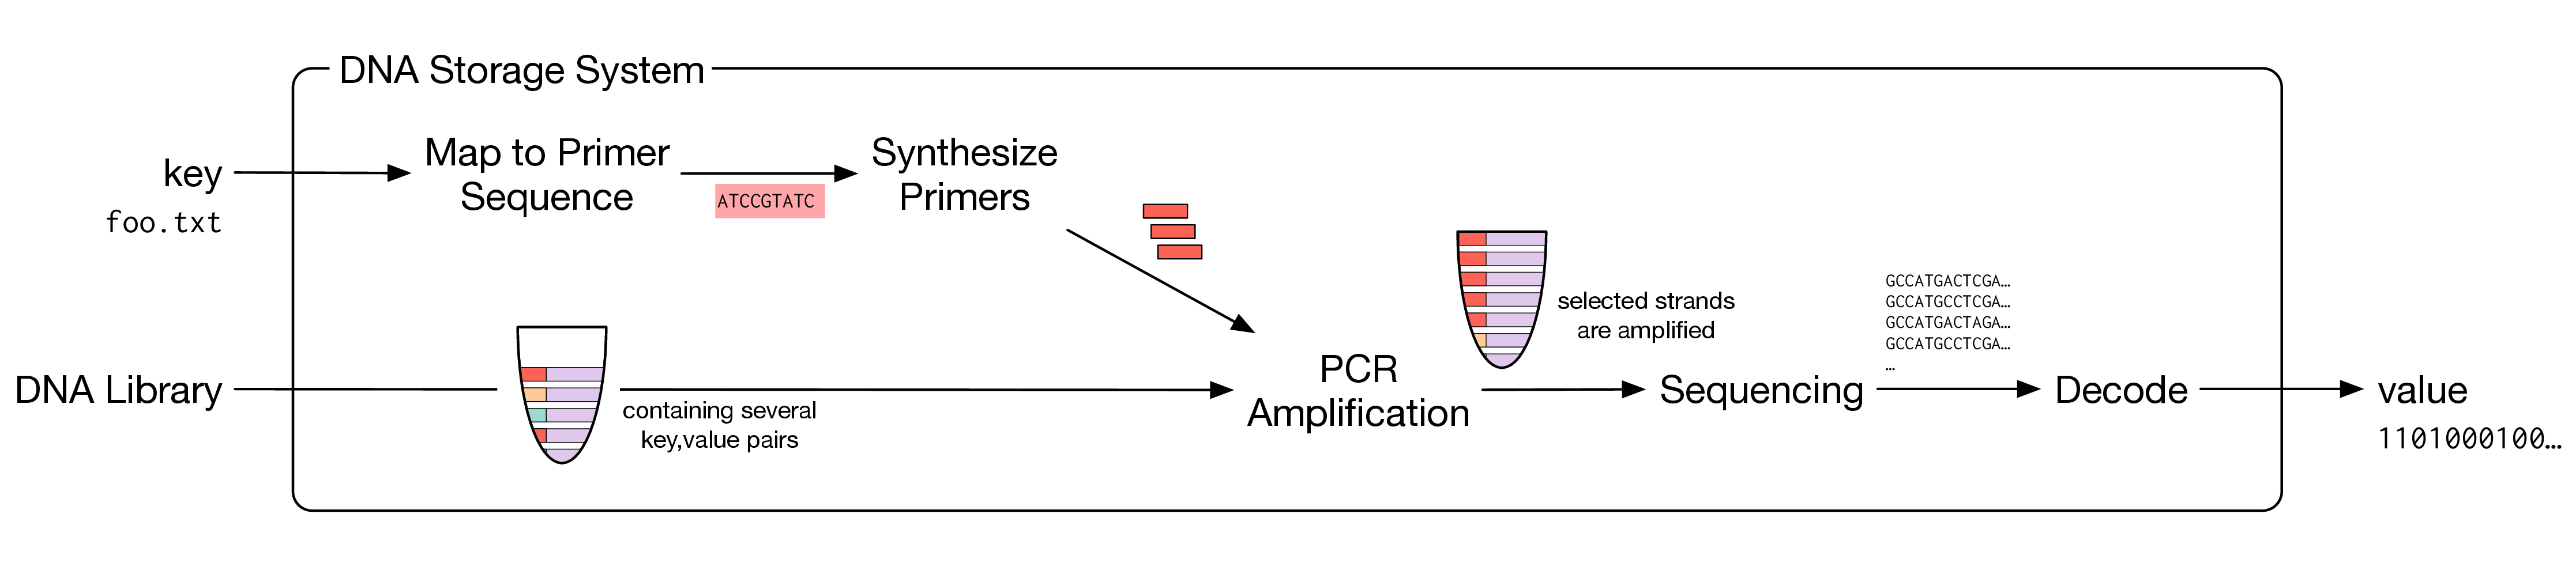
\includegraphics[width=1.1\textwidth]{images/read}
      \caption{DNA Storage System Read}
      \label{fig:read}
  \end{figure}

 Figure \ref{fig:write} shows flowcharts for the write (put) and Figure \ref{fig:read} read (get) processes in more detail. The write process (Fig. \ref{fig:write}) takes as input the key and value to store. It uses the key to obtain the PCR primer sequences, compute the high part of the address, and to determine the pool in the DNA library where the resulting strands will be stored. The low part of the address indexes the multiple strands generated by chunking the value (see Sec. 4.2). Next, it encodes the data addresses, payloads and error detection codes, and attaches the primer target sequences, to produce final DNA sequences for the synthesizer to manufacture. The resulting DNA molecules are stored in the storage library for archival.

 The read process (Fig. \ref{fig:read}) takes as input a key. It uses the key to obtain the PCR primer sequences that identify molecules in the pool associated with that key. Next, the storage system physically extracts a sample from the DNA pool that contains the stored data, but likely also includes large amounts of unrelated data. The sample and the PCR primers are sent to the PCR thermocycler, which amplifies only the desired strands. The resulting pool goes to the DNA sequencer, which ultimately produces the digital data readout. Note that this process might be iterative since it may require multiple samples and sequencing steps to extract all the data associated with the desired keys. The DNA synthesizer is used for both producing the DNA strands that hold data payload as well as synthesizing the PCR primers used to amplify data during the random access read process.

The read process removes a sample of DNA from the pool,and so cumulative reads reduce the quantity of DNA available for future operations. But DNA is easy to replicate, and so the pools can easily be replenished after read operations if necessary. If successive amplification is problematic, a pool can also be completely resynthesized after a read operation.

Researchers at Microsoft and the University of Washington have reached an early but important milestone in DNA storage by storing a record 200 megabytes of data on the molecular strands. The impressive part is not just how much data they were able to encode onto synthetic DNA and then decode. It’s also the space they were able to store it in. Once encoded, the data occupied a spot in a test tube “much smaller than the tip of a pencil.”
\subsection{Cell to Cell Communication}

Many viruses are capable of packaging and transmitting non-viral genetic material. For example, “transvestite” bacteriophage lambda particles can package and transduce phage T7 genomes or other genetic material. However, phage lambda and many viruses actively destroy the host cell in releasing virus particles.

Bacteriophage M13 (M13) is a filamentous phage whose progeny particles are secreted from infected cells.
M13 is selected as the cell-communicating virus. It’s the ideal specimen: It doesn’t kill the host cell, it is possible to vary the length of DNA that can be packed, and it can been engineered to get its DNA into mammalian cells. The M13 communication system is like a wireless information network for cells to send and receive messages. M13 wraps up strands of DNA (programmed by scientists) and sends them out in proteins that infect cells and release the DNA messages once they have gained entry. Scientists can send whatever they want in the DNA, everything from a sentence in a book to a sequence that encodes fluorescent protein. The M13 system dramatically increases the amount of data that can be transmitted at one time compared to previous cell-to-cell communication systems, roughly 80,000 bits compared to one bit with the sugar molecule system. M13 can also transmit data over long ranges. The technology could be used in tissue engineering as well as in creating artificial organs and biomaterials that have no direct analog in nature. This is referred to as ``Biological Internet''.

\subsection{Transcriptor - Biological Transistor}

A biological transistor is made from genetic material — DNA and RNA — in place of gears or electrons. The team calls its biological transistor the “transcriptor". The biological transistor developed by Jerome Bonnet and colleagues could be used inside living cells to record when cells have been exposed to certain external stimuli, or even to turn on and off cell reproduction as needed. The creation of the transcriptors enable bio computers to study and reprogram living systems, monitors environments and improve cell therapeutics.

In electronics, a transistor controls the flow of electrons along a circuit. Similarly, in biologics, a transcriptor controls the flow of a specific protein, RNA polymerase, as it travels along a strand of DNA. A group of natural proteins, called integrases, is repurposed to realize digital control over the flow of RNA polymerase along DNA, which in turn allowed to amplify genetic logic. Using transcriptors, it is possible to create what is known in electrical engineering as logic gates that can derive true-false answers to virtually any biochemical question that might be posed within a cell. These transcriptor-based logic gates as “Boolean Integrase Logic,” or “BIL gates” for short. Transcriptor-based gates alone do not constitute a computer, but they are the third and final component of a biological computer that could operate within individual living cells.

“AND” and “OR” are just two of the most basic Boolean logic gates. An “AND” gate, for instance, is “true” when both of its inputs are true — when “a” and “b” are true. An “OR” gate, on the other hand, is true when either or both of its inputs are true. In a biological setting, the possibilities for logic are as limitless as in electronics, it is possibleto test whether a given cell had been exposed to any number of external stimuli — the presence of glucose and caffeine, for instance. BIL gates will make that determination and  store that information so that it could easily identify those which had been exposed and which had not. By the same token, it  can command the cell to start or stop reproducing if certain factors were present. And, by coupling BIL gates with biological Internet, it is possible to communicate genetic information from cell to cell to orchestrate the behavior of a group of cells. The transcriptor achieves a key similarity between the biological transistor and its semiconducting cousin: signal amplification.


\section{Comparison with Conventional Computers}

\textbf{Similarities}

  \begin{itemize}
    \item \textbf{Transformation of Data}

        Both DNA computers and electronic computers use Boolean logic (AND, OR, NAND, NOR) to transform data. The logical command ``AND'' is performed by separating DNA strands according to their sequences, and the command ``OR'' is done by pouring together DNA solutions containing specific sequences. For example, the logical statement ``X or Y'' is true if X is true or if Y is true. To simulate that, the scientists would pour the DNA strands corresponding to ``X'' together with those corresponding to ``Y''. Following is an example of how a Bio Chemical Inverter works.
       Working of inverter, the concentration of a particular messenger RNA (mRNA) molecule represents a logic signal. In the first case, the input mRNA is absent and the cell transcribes the gene for the output mRNA using RNA polymerase (RNAp) molecules. In the second case, the input mRNA is present and the cell translates the input mRNA into the input protein using ribosomes.
      A digital inverter that consists of a gene encoding the instructions for protein B and containing a region (P) to which protein A binds. When A is absent (left)—a situation representing the input bit 0, the gene is active and B is formed—corresponding to an output bit 1. When A is produced (right)—making the input bit 1, it binds to P and blocks the action of the gene—preventing B from being formed and making the output bit 0.

      \item \textbf{Manipulation of Data}

      Electronic computers and DNA computers both store information in strings, which are manipulated to do processes. Vast quantities of information can be stored in a test tube. The information could be encoded into DNA sequences and the DNA could be stored. To retrieve data, it would only be necessary to search for a small part of it - a key word, for example – by adding a DNA strand designed so that its sequence sticks to the key word wherever it appears on the DNA.

      \item \textbf{Computation Ability}

      All computers manipulate data by addition and subtraction. A DNA computer should be able to solve a satisfiability problem with 70 variables and 1,000 AND-OR connections. To solve it, assign various DNA sequences to represent 0’s and 1’s at the various positions of a 70 digit binary number. Vast numbers of these sequences would be mixed together, generating longer molecules corresponding to every possible 70-digit sequence 
  \end{itemize}


\hspace{-12pt}\textbf{Differences}
\\ 
\begin{table}[h!]
\begin{center}{
\begin{tabular}{| m{7em} | m{4cm} | m{4cm} | }
  \hline
  \textbf{} & \textbf{Conventional} & \textbf{Biological}\\
  \hline
  \textbf{Components and Materials} & Inorganic, e.g. silicon & Biological, e.g.DNA\\ 
  \hline
  \textbf{Data representation} & Base 2  & Base 4\\
  \hline
  \textbf{Size} & Large & Small\\
  \hline
   % \textbf{Maximum Operations} & \rule{0pt}{5ex} 10^\textsuperscript{12} op.s/sec. & \rule{0pt}{5ex}10^\textsuperscript{14} op.s/sec.\\
  % \hline
  \textbf{Processing scheme} & Sequential and limited massively parallel & Massively parallel\\
  \hline
  \textbf{Toxic components?} & Yes & No\\
  \hline
  \textbf{Energy efficient?} & No & Yes\\
  \hline
\end{tabular}
}
\caption{Table to test captions and labels}
\label{table:1}
\end{center}
\end{table}

\section{Advantages and Disadvnatages of bio compters}

\textbf{Advantages}

\begin{itemize}
    \item {Performs millions of operations at same time.
          \begin{itemize}
        \item{Good for parallel computing.}
      \end{itemize}
            }
        \item {Ability to use large amounts of working memory.
          \begin{itemize}
        \item{1 gram of DNA can hold 1 x 1014 MB of data Or 145 trillion CDs.}
                \item{1 CD is 800 MB.}
      \end{itemize}
            }
       
    \item {Cheaper.}
        \item {Lightweight.
          \begin{itemize}
        \item{1 lb of DNA has more computing power than all computers ever made.}
      \end{itemize}
            }
    \item { Low power used to keep in original state.}
    \item {Has ability to solve hardest problems in a matter of weeks.}
        \item {Environmentally friendly.
          \begin{itemize}
        \item{Clean, readily available materials.}
      \end{itemize}}
  \end{itemize}


  % \hspace{-12pt}
  \textbf{Disadvantages}

    \begin{itemize}
    \item {Molecular operations are not perfect.}
    \item {DNA computing involves a relatively large amount of error.}
    \item {As size of problem grows, probability of receiving incorrect answer eventually becomes greater than probability of receiving correct answer.}
    \item {Sometimes there are errors in the pairing of DNA strands.}
        \item {Simple problems solved faster on electronic computers.}
    \item {Human assistance is required.}
    \item {No universal method of data representation.}
    \item {Time consuming lab procedures.}
        \item {DNA has a half-life.
          \begin{itemize}
        \item{Solutions could dissolve away before end result is found.}
      \end{itemize}
            }
        \item {Information can be untransmittable.
          \begin{itemize}
        \item{Current DNA algorithms compute successfully without passing any information from one processor to the next in a multiprocessor connection bus.}
      \end{itemize}
            }
  \end{itemize}

\section{Applications}

\subsection{Medical Application}

Biological computers are made inside a patient’s body. The mere information of the patient’s body is called a blueprint along which lines the biological computer would be manufactured. Once the computer’s genetic blueprint has been provided, the human body will start to build it on its own using the body’s natural biological processes  and the cells found in the body. Through boolean logic equations, we can easily use the biological computer to identify all types of cellular  activity and determine whether a particular activity is harmful or not. The cellular activities that the biological computer could detect can even include those of mutated genes and all other activities of the genes found in cells. As with conventional computers, the biological computer also works with an output and an input signal. The main inputs of the biological computer are the body’s proteins, RNA and other specific chemicals that are found in the human cytoplasm. The output on the other hand could be detected using laboratory equipment.

\subsection{Solving NP-Problems} % (fold)
\label{sub:subsection_name}
The primary advantage offered by most proposed models of DNA based computation is the ability to handle millions of operations in parallel. The massively parallel processing capabilities of DNA computers may give them the potential to find tractable solutions to otherwise intractable problems, as well as potentially speeding up large, but otherwise solvable, polynomial time problems requiring relatively few operations.

A working DNA based computer might hold an advantage over conventional computers when applied to decomposable problems, those problems that are able to be divided into separate, non-sequential tasks, because they can hold so much data in memory and conduct so many operations at once. However, due to the length of time required to conduct the biochemical operations, non-decomposable problems, those requiring many sequential operations, are likely to remain much more efficient on a conventional computer. 
% subsection subsection_name (end)
\subsection{Cryptography} % (fold)
\label{sub:subsection_name}
 DNA computing techniques have already been theoretically applied to a real life problem: breaking the Data Encryption Standard (DES). Although this problem has already been solved using conventional techniques in a much shorter time than proposed by the DNA methods, the DNA models are much more flexible, potent and  cost effective.

DES is a method of encrypting 64-bit messages with a 56-bit key, used extensively in the United States. Electronic keys are normally a string of data used to code and/or decode sensitive messages. By finding the appropriate key to a set of encrypted messages, one can either read encoded messages or pose as the such messages. Using a special purpose electronic computer and differential cryptanalysis, it has been shown that the key to DES can be found in several days. However, to do so would require 2\textsuperscript{43} examples of corresponding encrypted and unencrypted messages (known as plain-text/cipher-text pairs) and would slow down by a factor of 256 if the strength of the encrypting key was increased to 64-bits. It is proposed that DES could be broken using a DNA based computer and a search algorithm similar to Adleman's original technique. This procedure would be expected to take 4 months, but would only need a single plain-text/cipher-text pair or an example of cipher text with several plain text candidates to be successful. The feasibility of applying DNA computation to this problem was also addressed  using a more refined algorithm (the sticker model approach) which enabled the researchers to suggest that they could solve the problem using less than a gram of DNA, an amount that could presumably be handled by a desk top sized machine. Both models would likely be more cost and energy effective than the expensive electronic processors required by conventional means, but are entirely theoretical. The first model ignores error rates incurred though laboratory techniques and the inherent properties of the DNA being used. The second model requires an error rate approaching .0001, with higher rates substantially affecting the volume of DNA required. Despite these assumptions, these models show that existing methods of DNA computation could be used to solve a real life problem in a way that is both practical and superior to methods used by conventional computers. It is also demonstrated that such benefits can be obtained despite error rates that would be unacceptable in an electronic computer and that may be unavoidable in a molecular one.

% subsection subsection_name (end)
\newpage
\section{Conclusion}

While  a  desktop  PC  is  designed  to  perform  one  calculation  very  fast, DNA  strands  produce  billions  of  potential  answers  simultaneously. This  makes  the  DNA  computer  suitable  for  solving  ``fuzzy  logic'' 
problems that have many possible solutions rather than the either/or logic of binary computers. In the future, some speculate, there may be hybrid  machines  that  use  traditional  silicon  for  normal  processing 
tasks  but  have  DNA  co-processors  that  can  take  over  specific  tasks they would be more suitable for. 

Implanting computer programs into living creatures may not be far away. In the past few years, scientists have taken the first steps towards creating a host of cellular robots that are programmed to carry out tasks such as detecting and cleaning up environmental pollutants, tracking down cancer cells in a body and manufacturing antibiotics or molecular-scale electronic components. These researchers have imported notions of electrical engineering—digital logic, memory and oscillators—into the realm of biology.
\newpage
\begin{thebibliography}{9}
  \bibitem{nano3}
  Leonard  M.  Adleman, 
  ``Computing  with  DNA,''
    \emph{Scientific  American, August 1998.}
  
  \bibitem{nano3}
  T Jeevani, 
  ``Biological computer - their mechanism and applications,'' 
  \emph{Journal of Biotechnology and Biomaterials, 2011.}
    \bibitem{nano3}
  L.Adleman, ``On  constructing  a  molecular  computer,'' 
  \emph{1st  DIMACS  workshop  on  DNA  based  computers,  Princeton,  1995.  In  DIMACS series, vol.27, 1996.}
\bibitem{nano3}
  Monica E Ortiz and Drew Endy,
  ``Engineered cell-cell communication via DNA messaging,''
  \emph{Journal of Biological Engineering, 2012.}
\bibitem{nano3}
  Robert T. Gonzalez, 
  ``This new discovery will finally allow us to build biological computers,''
  \emph{IO9. Retrieved March 29, 2013.}
\bibitem{nano3}
  Braich, Ravinderjit S. ,
  ``Solution of a satisfiability problem on a gel-based DNA computer,''
  \emph{DNA Computing. Springer Berlin Heidelberg, 2001.}
 \bibitem{nano3}
	Stanford creates biological transistors, the final step towards computers inside living cells.
  \emph{http://www.extremetech.com}
\end{thebibliography}  
\end{document}
